%------------------------------------------------------------
%------------------------------------------------------------
\subsection{Rules}
\label{sec:rules}
%For instance, unconditional start time restrictions using predicates such as {\SAMEDAILYSLOT} or {\FORBIDDENPERIOD}  may be enforced on any set of sessions bound to a course, a part, a class or more generally to the course domain. Conversely, start time restrictions on a set of sessions bound to a resource will only be enforced on those which are eventually assigned to the resource.
%Predicates serve to constrain the possible sessions of resources (e.g., unavailabilities of a teacher) or the constitutive sessions of course elements (e.g., periodicity of a class). 
%e-maps may then be adjusted to constrain candidate sessions of resources (e.g., teacher unavailability), constitutive sessions of course elements (e.g., class periodicity), or individual sessions (e.g., session sequencing and parallelization).
Rules are used to state conjunctions of constraints and in particular single constraints. %and in particular individual (singleton) constraints.
Each rule is defined by a universally quantified formula which restricts the domains of the e-map variables of a given predicate.
The collection of constraints hence represented is obtained by instantiating the predicate with each tuple of e-maps belonging to the cross-product of the domains.
E-map domains are not given in extension
but represented using a language of selectors
which provides a comprehension syntax to generate and filter e-maps.
Let 
${\SELECTOR}$
denote the language of e-map domain selectors,
%(${\SELECTOR}\subseteq({\TYPE}\times{\LABEL}\times{2^{\RANK}})^{n}$).
a {\UTP} rule has the form %is a tuple 
\begin{align}
c(F_1,\ldots,F_m,p_1,\ldots,p_n)
\end{align}
and is interpreted by %The semantics of a rule $(c,D_1,\ldots,D_m,p_1,\ldots,p_n)$ is 
the %quantified 
formula
\begin{multline}
\forall (e_1,S_1)\in\denote{F_1},\ldots,(e_m,S_m)\in\denote{F_{m}}:\\
c((e_1,S_1),\ldots,(e_m,S_m),p_1,\ldots,p_n)
\label{rule:rule}
\end{multline}
where 
$c$ is a predicate symbol of arity $m$,
$F_1,\ldots,F_m$ are selectors ($F_i\in{\SELECTOR}$, $i=1\ldots m$),
$p_1,\ldots p_n$ are values for the parameters of $c$ ($n\geq0$),
and
$\denote{F_i}$
denotes the domain of e-maps represented by
selector 
$
F_i\in{\SELECTOR}
$
.

The language of selectors allows 
to target entities based on type, label or identity
and
to filter their sets of sessions
based on session rank and mutual compatibility with other entities.
It is complete in the sense 
that it allows to construct any domain of e-maps whose entities share the same type.
For instance, one may construct the e-maps which
associate any of the rooms labeled \texttt{Building-A}
with the compatible sessions of rank 2 or 4 
that are also constitutive of course \texttt{course-1} or class \texttt{class-3}.
A selector
combines a generator and an optional list of filters.
Generators and filters are triples 
$
(T_i,L_i,O_i)
$
consisting of
an entity type
$
T_i%\in{\TYPE}
$,
an entity label or identifier
$
L_i%\in{\LABEL}
$
and
a subset of session ranks
$
O_i%\subseteq{\RANK}
$ (a.k.a., session mask),
the latter two elements being optional.
A selector 
matches any e-map
whose entity satisfies the type, label and identifier constraints of the generator
and whose %set of sessions 
image includes any compatible session
satisfying the mask of the generator
and one of the filters.
Note that rules featuring empty selectors are discarded during the flattening stage. 
%Selectors are encoded as attributes in the {\XML} language
%using a syntax that borrows from the CSS selector language.
%For instance, the above example would be encoded by the following XML fragment: 
%\todo[inline]{Marc : Rajouter une phrase pour décrire brièvement la figure 3}

\begin{figure*}[h]
\centering
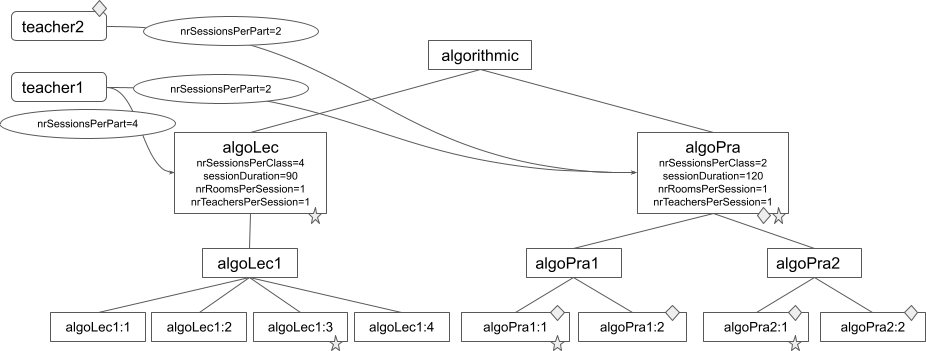
\includegraphics[scale=0.5]{img/utp_rule_1.png}
\caption{Rule interpretation}
\label{fig:utp-rule-1}
\end{figure*}

%\marc{Mettre ici le dernier paragraphe sur la sélection des rangs ? Et l'exemple en fin de section ?}
Let
${\RANK}$
denote the range of session ranks,
${\maptype{\RANK}{\SESSION}}:\RANK\rightarrow2{^\SESSION}$
the rank-based partitioning of sessions,
and
${\LABEL}$
the set of labels 
(${\LABEL}\subseteq2^{{\ENTITY}}$)
completed 
with the whole set of entities to mock label optionality
($\ENTITY\in{\LABEL}$)
and singleton entities to support identity-based selection
($\myset{\myset{e}\ |\ e\in{\ENTITY}}\subseteq{\LABEL}$),
the language of selectors
is the set 
$
\cup_{n\geq1}({\TYPE}\times{\LABEL}\times{2^{\RANK}})^{n}
$.
%where each 
Each selector 
$
d=((T_1,L_1,O_1),\ldots,(T_k,L_k,O_k))
$
%($k\geq1$)
decomposes into a generator
$
(T_1,L_1,O_1)
$
and a possibly empty list of filters
$
((T_2,L_2,O_2),\ldots,(T_k,L_k,O_k))
$.
%A session $s$ is said to satisfy triple
%$
%(T_i,L_i,O_i)
%%\in({\TYPE}\times{\LABEL}\times{2^{\RANK}})
%$
%if
%it is compatible with
%an entity of type $T_i$ and label $L_i$ 
%($s\in\map{T_i}{\SESSION}{L_i}$)\footnote{
%%Let $X\subseteq Y$,
%$
%{\map{Y}{\SESSION}{X}}
%$
%denotes
%$
%\setunion{i}{X\cap Y}{\map{Y}{\SESSION}{i}}
%$.
%}
%and 
%if it satisfies mask $O_i$, i.e., its rank is included in $O_i$
%($s\in\map{\RANK}{\SESSION}{O_i}$).
%A selector 
%$
%d=((T_1,L_1,O_1),\ldots,(T_k,L_k,O_k))
%$
$d$ matches any e-map
whose entity has type $T_1$ and label $L_1$ and whose image includes any compatible session satisfying mask $O_1$ and any of the filters.
The set of e-maps
$\denote{d}$
matched by $d$
%selector 
%$
%d%=
%%((T_1,L_1,O_1),\ldots,(T_k,L_k,O_k))
%$
%represents
%the set of e-maps 
is defined by
\begin{multline*}
\denote{d}=
\bigcup\limits_{e\in{T_1}}
%\myset\left\{(e,S')
\Big \{(e,S')
\ |\ 
%e\in T_1\cap L_1,
S'=
\mape{T_1}{\SESSION}{\myset{e}\cap L_1}
%\cap 
%\map{\RANK}{\SESSION}{O_1}
\;\cap \\
\bigcup\limits_{i=2\ldots k}
{
\mape{T_i}{\SESSION}{L_i}
\cap
\mape{\RANK}{\SESSION}{O_1\cap O_i}
\wedge
S'\neq\emptyset
}
\Big \}
\end{multline*}

where
$
{\mape{X}{Y}{X'}}
=
%$
%denotes
%$
\bigcup\limits_{i\in X'}{\map{X}{Y}{i}}
$
with
$X'\subseteq X$
.

Figure~\ref{fig:utp-rule-1} is a toy example to illustrate the interpretation of rules.
The course \texttt{algorithmic} has 2 parts : lecture part \texttt{algoLec} and practice part \texttt{algoPra}.
There is 1 lecture class, taught by \texttt{teacher1}, and 2 practical classes taught by \texttt{teacher1} and \texttt{teacher2}.
%\todo[inline]{Marc : harmoniser notations}
The lecture class has 4 sessions and each practical class has 2 sessions.
Figure~\ref{fig:utp-rule-1} illustrates the flattening of the following rules: 
%on a simple model consisting of 2 teachers and & course subdivided into 2 parts, 3 classes and 8 sessions. The first rule forbids a time period for 

{\footnotesize{
\begin{multline}
\texttt{\mbox{\hspace*{-1em}}{\FORBIDDENPERIOD}((<(\TEACHER,{teacher2},\_)>,9120,9240)}\label{rule-example-1}\\
\end{multline}
\begin{multline}
\texttt{\mbox{\hspace*{-1em}}{\SEQUENCED}(<(\CLASS,\_,\myset{3}),(\PART,{algoLec},\_)>,}\\
\texttt{<(\CLASS,\_,\myset{1}),(\PART,{algoPra},\_)>)\label{rule-example-2}}
\end{multline}
}}

Rule~\ref{rule-example-1}
requires that \texttt{teacher2} has no session between 8am and 10am the second day of week 2.
In this example, the time grid has 1440 slots a day and 5 days a week, meaning that slot %value\footnote{Each possible session slot is mapped to a single value. All possible values make up the domain of a session.} 
9120 (resp. 9240) corresponds to 8am (resp. 10am) the second day of week 2.
The selector includes no mask and no filter hence matches with all possible sessions of \texttt{teacher2} 
as indicated with diamonds on Figure~\ref{fig:utp-rule-1}. 
The resulting domain of e-maps is the singleton $\myset{(teacher2,\map{\TEACHER}{\SESSION}{teacher2})}$
and the rule is flattened into a single \texttt{\FORBIDDENPERIOD} constraint. %$\myset{\map{\TEACHER}{\SESSION}{teacher2}}$.
Rule~\ref{rule-example-2}
%requires that the first practical session in Algorithmic \todo[inline]{Marc : pourquoi algo ?} start after the third lecture.
requires that the first sessions of the practices start after the third session of the lecture.
The two selectors include a filter. The first selector matches with all class sessions of rank 3 in part \texttt{algoLec}, 
and the second matches with all class sessions of rank 1 in part \texttt{algoPra} as indicated with stars on the figure.
The rule is flattened into 2 \texttt{\SEQUENCED} constraints corresponding to the cross product of the e-map domains $\myset{(algoLec1,\map{\RANK}{\SESSION}{3}\cap\map{\PART}{\SESSION}{algoLec})}$
and $\myset{(algoPra1,\map{\RANK}{\SESSION}{1}\cap\map{\PART}{\SESSION}{algoPra}),(algoPra2,\map{\RANK}{\SESSION}{1}\cap\map{\PART}{\SESSION}{algoPra})}$.
